% ============================================================
%  DSP391m - Nhóm 5 | Báo cáo tiến độ - Phase 2: Benchmarking
%  Sinh tự động từ reports/tables/*.csv bởi tools/build_progress_deck.py
%  KHÔNG sửa số liệu trong file này - chạy lại builder sau mỗi renumber.
%  Compile: tectonic Progress_Report_Slides.tex   (XeTeX, font Noto Sans)
% ============================================================
\documentclass[aspectratio=169,11pt]{beamer}
\usetheme{default}
\setbeamertemplate{navigation symbols}{}
\usepackage{fontspec}
\setmainfont{Noto Sans}
\setsansfont{Noto Sans}
\usepackage{booktabs}
\usepackage{graphicx}
\graphicspath{{../figures/}}

\definecolor{themecol}{HTML}{0F4C81}
\definecolor{accent}{HTML}{C0392B}
\definecolor{rowtint}{HTML}{EEF3F8}
\setbeamercolor{structure}{fg=themecol}
\setbeamercolor{frametitle}{fg=white,bg=themecol}
\setbeamercolor{title}{fg=themecol}
\setbeamerfont{frametitle}{series=\bfseries,size=\large}
\setbeamertemplate{itemize item}{\color{themecol}\textbullet}
\setbeamertemplate{footline}{\hfill\scriptsize\color{gray}%
  DSP391m · Nhóm 5 · Phase 2 Benchmarking\quad\insertframenumber/\inserttotalframenumber\hspace{2mm}\vspace{1mm}}

\title{Time-Aware Explainable ML —\\Phát hiện sớm sinh viên nguy cơ (OULAD)}
\subtitle{Báo cáo tiến độ · Phase 2 — Benchmarking mô hình}
\author{Ngọc Sang (Modeling Lead) — Nhóm 5 · GVHD: Phan Duy Hùng}
\institute{Đại học FPT · DSP391m}
\date{}

\begin{document}

\begin{frame}\titlepage\end{frame}

\begin{frame}{Lựa chọn mô hình — vì sao 5 thuật toán này?}
\small
\begin{tabular}{@{}lll@{}}
\toprule
\textbf{Model} & \textbf{Họ thuật toán} & \textbf{Lý do chọn} \\
\midrule
Logistic Regression & Tuyến tính & Baseline chuẩn, hệ số đọc được trực tiếp \\
Random Forest & Bagging cây & Bền với nhiễu/ngoại lai, ít phải tinh chỉnh \\
XGBoost & Boosting cây & SOTA dữ liệu bảng, hỗ trợ SHAP TreeExplainer \\
LightGBM & Boosting cây & Nhanh trên dữ liệu lớn, đối chứng cùng họ \\
ANN (MLP) & Mạng nơ-ron & Đại diện phi tuyến khác họ cây \\
\bottomrule
\end{tabular}
\vspace{4mm}
\begin{itemize}
  \item Phủ \textbf{3 họ mô hình} (tuyến tính · cây · nơ-ron) → kết luận không lệ thuộc một họ.
  \item Cả 5 đều xuất hiện trong các nghiên cứu nền trên OULAD → \textbf{so sánh được với văn liệu}.
\end{itemize}
\end{frame}

\begin{frame}{Kiến trúc \& cấu hình huấn luyện}
\small
\begin{tabular}{@{}ll@{}}
\toprule
\textbf{Model} & \textbf{Cấu hình chính (còn lại giữ mặc định)} \\
\midrule
Logistic Regression & \texttt{max\_iter=1000} \\
Random Forest & mặc định · \texttt{n\_jobs=-1} \\
XGBoost & \texttt{tree\_method=hist} · \texttt{eval\_metric=logloss} \\
LightGBM & mặc định · \texttt{verbose=-1} \\
ANN (MLP) & 2 lớp ẩn (64, 32) · \texttt{max\_iter=500} · early-stopping \\
\bottomrule
\end{tabular}
\vspace{4mm}
\begin{itemize}
  \item \textbf{Cùng seed 42} cho mọi model → công bằng \& tái lập.
  \item Giai đoạn so tuyển \emph{chưa} tinh chỉnh siêu tham số — chọn xong ứng viên mới tune.
\end{itemize}
\end{frame}

\begin{frame}{Quy trình huấn luyện (Training Procedure)}
\begin{enumerate}
  \item Nạp \textbf{split cố định} của mốc 100\% — 0 sinh viên trùng train/test, toàn bộ kiểm thử rò rỉ tự động ĐẠT.
  \item Tiền xử lý \textbf{fit trên train} → transform test (median, winsorize, encoder, scaler đều học từ train).
  \item \texttt{model.fit(train)} → dự đoán trên \textbf{test giữ riêng}.
  \item Chấm \textbf{7 chỉ số}; xếp hạng theo \textbf{recall} lớp at-risk.
\end{enumerate}
\vspace{3mm}
\begin{itemize}
  \item Bảng kết quả trình bày \textbf{baseline no-resample}; pipeline chuẩn giữ SMOTE theo proposal — Phase 4 chứng minh hai lựa chọn chênh không đáng kể.
  \item Chỉ số chính: \textbf{recall \& PR-AUC} lớp at-risk — bỏ sót một sinh viên nguy cơ đắt hơn nhiều một cảnh báo nhầm.
\end{itemize}
\end{frame}

\begin{frame}{Kết quả so tuyển @ mốc 100\%}
\centering
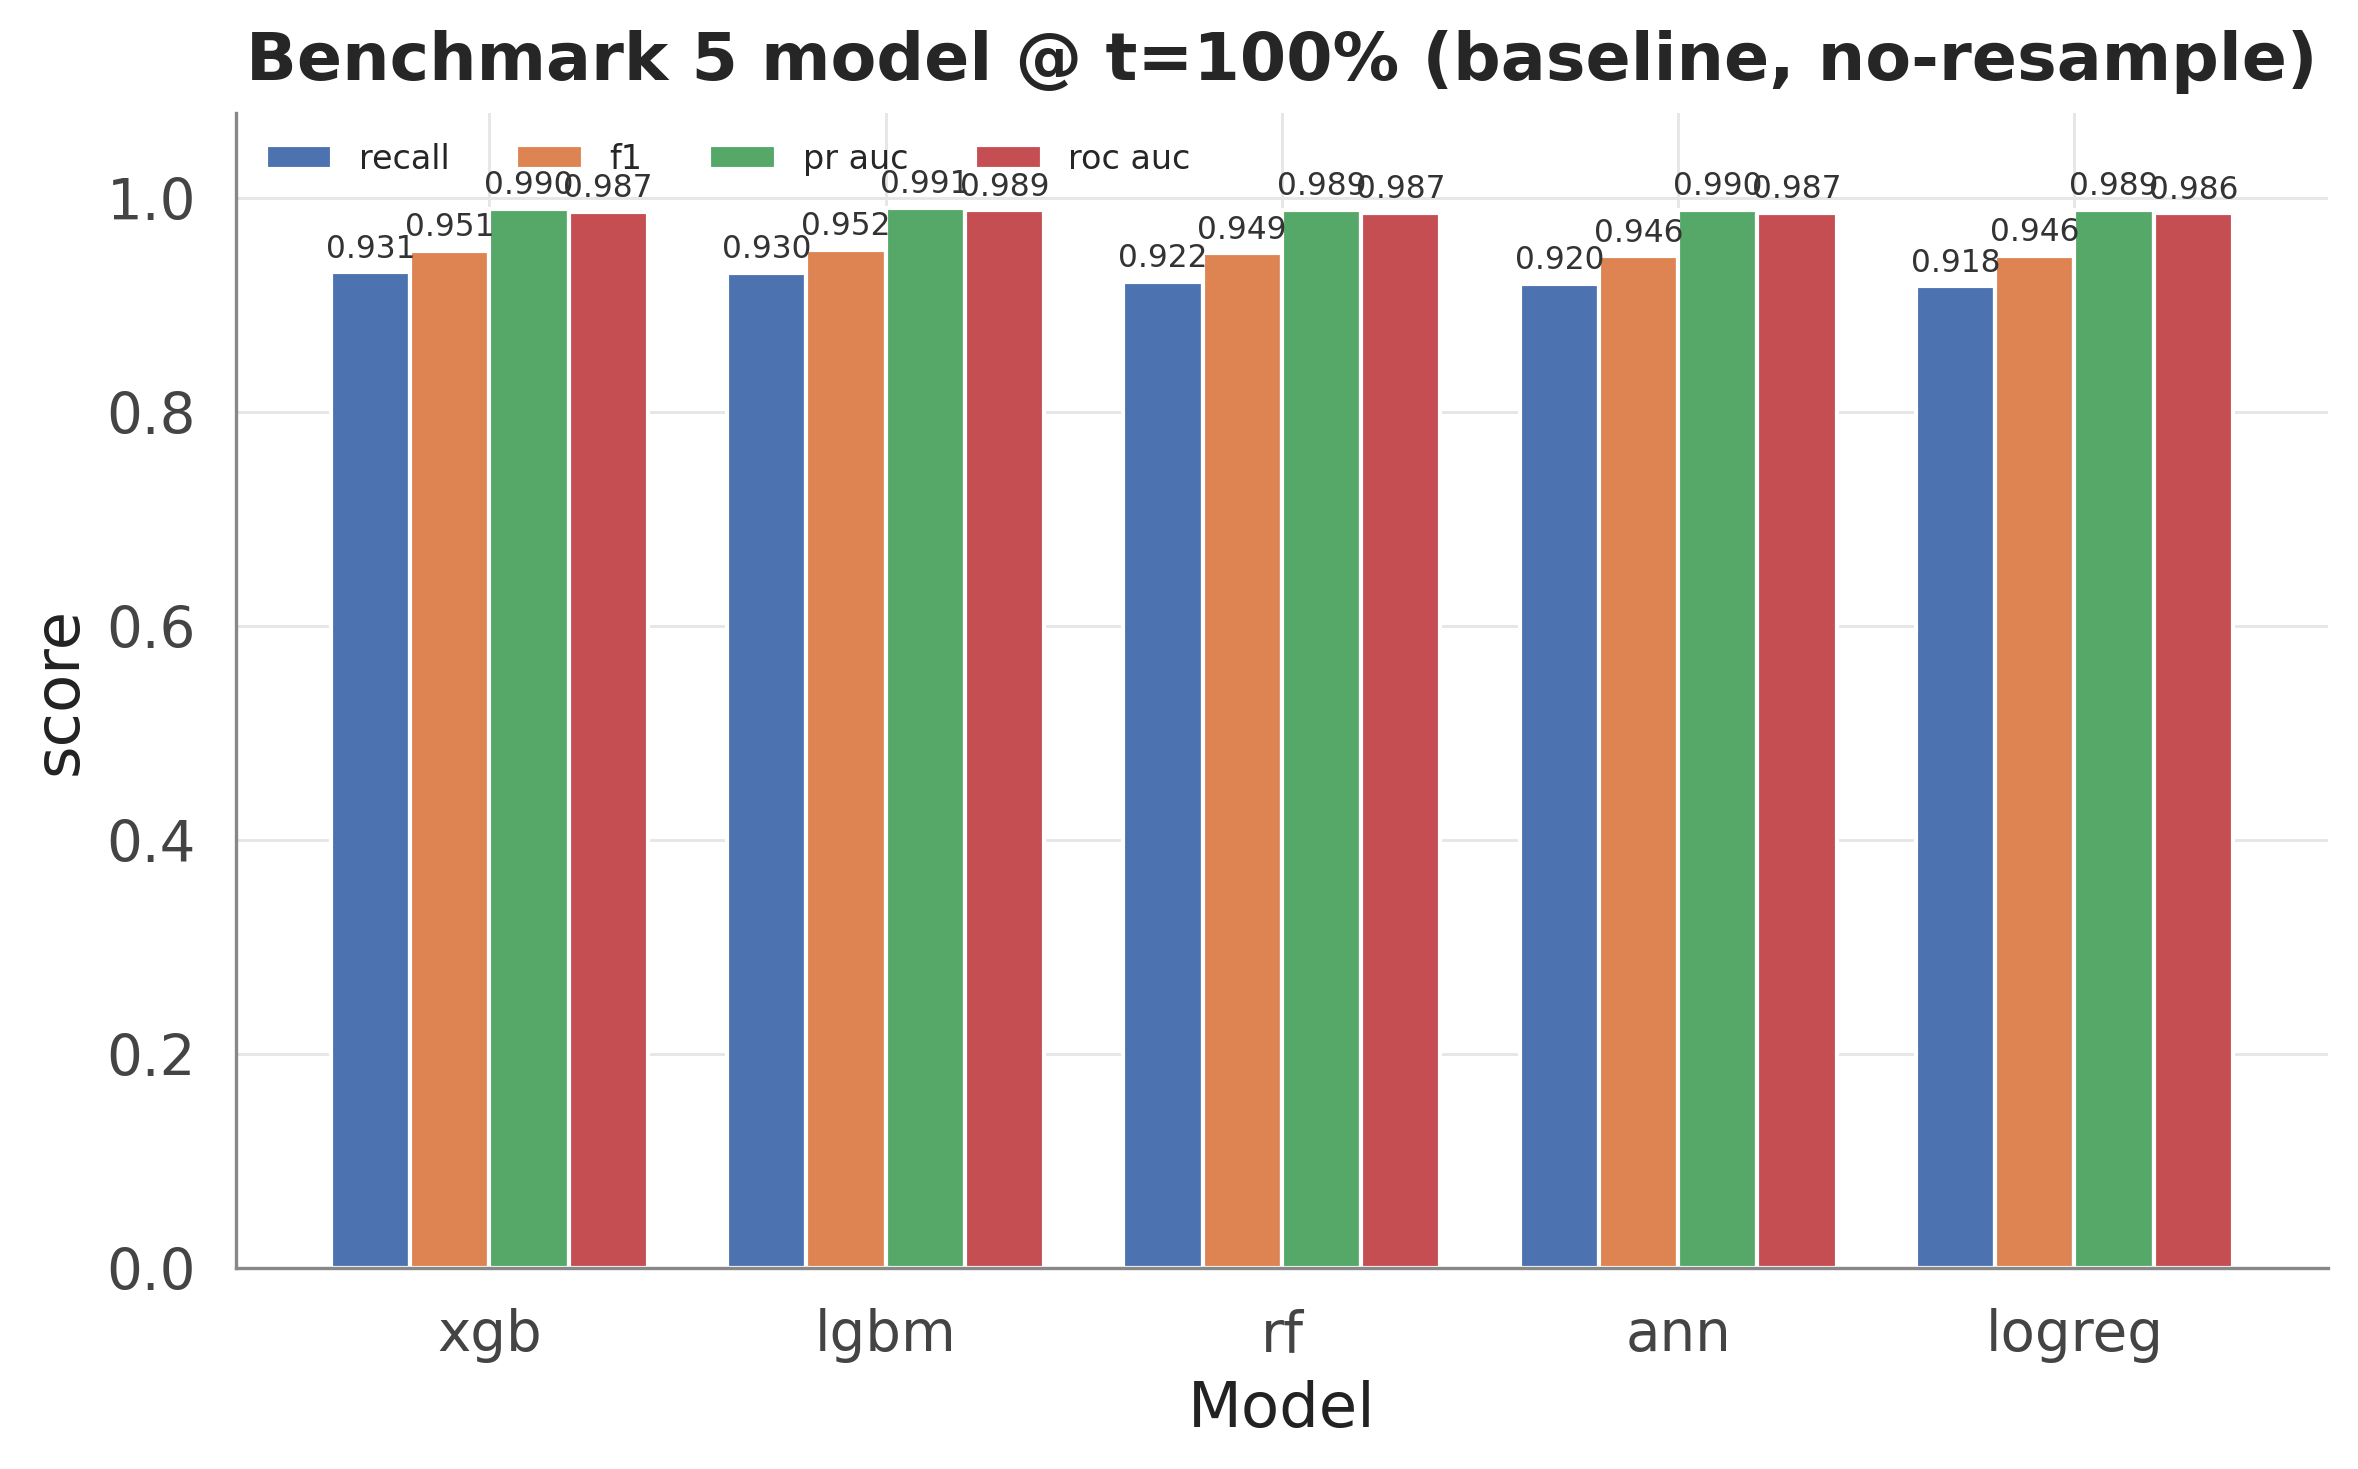
\includegraphics[height=0.82\textheight]{model_benchmark_baseline.png}
\end{frame}

\begin{frame}{Bảng hiệu năng đầy đủ — 7 chỉ số (sinh từ CSV)}
\centering\small
\textbf{XGBoost}: recall \textbf{0.931} · F1 \textbf{0.951} · PR-AUC \textbf{0.990} · Brier 0.038 (thấp = tốt)\\[2mm]
\begin{tabular}{@{}lcccccc@{}}
\toprule
\textbf{Model} & \textbf{Recall} & \textbf{F1} & \textbf{PR-AUC} & \textbf{ROC-AUC} & \textbf{Precision} & \textbf{Brier}$\downarrow$ \\
\midrule
    XGBoost & 0.931 & 0.951 & 0.990 & 0.987 & 0.972 & 0.038 \\
    LightGBM & 0.930 & 0.952 & 0.991 & 0.989 & 0.974 & 0.037 \\
    Random Forest & 0.922 & 0.949 & 0.989 & 0.987 & 0.977 & 0.041 \\
    ANN (MLP) & 0.920 & 0.946 & 0.990 & 0.987 & 0.973 & 0.041 \\
    Logistic Regression & 0.918 & 0.946 & 0.989 & 0.986 & 0.976 & 0.041 \\
\bottomrule
\end{tabular}
\vspace{3mm}
\begin{itemize}\small
  \item Test giữ riêng, baseline no-resample; khoảng cách giữa các model \textbf{nhỏ} → hai slide sau kiểm chứng độ tin cậy.
\end{itemize}
\end{frame}

\begin{frame}{Độ tin cậy: CV 5-fold $\times$ 5 seed trên train}
\centering\small
\begin{tabular}{@{}lccc@{}}
\toprule
\textbf{Model} & \textbf{Recall ($\mu\pm\sigma$)} & \textbf{F1 ($\mu\pm\sigma$)} & \textbf{PR-AUC ($\mu\pm\sigma$)} \\
\midrule
    XGBoost & 0.9309 $\pm$ 0.0047 & 0.9507 $\pm$ 0.0032 & 0.9901 $\pm$ 0.0008 \\
    LightGBM & 0.9295 $\pm$ 0.0060 & 0.9516 $\pm$ 0.0036 & 0.9907 $\pm$ 0.0008 \\
    ANN (MLP) & 0.9245 $\pm$ 0.0081 & 0.9463 $\pm$ 0.0038 & 0.9891 $\pm$ 0.0009 \\
    Random Forest & 0.9202 $\pm$ 0.0051 & 0.9489 $\pm$ 0.0030 & 0.9889 $\pm$ 0.0009 \\
    Logistic Regression & 0.9180 $\pm$ 0.0054 & 0.9452 $\pm$ 0.0033 & 0.9887 $\pm$ 0.0010 \\
\bottomrule
\end{tabular}
\vspace{3mm}
\begin{itemize}\small
  \item 25 lần fit/model, tiền xử lý + cân bằng lặp \textbf{trong từng fold} — không rò rỉ.
  \item $\sigma$ rất nhỏ → kết quả \textbf{ổn định}, không ăn may theo cách chia fold; thứ hạng CV khớp thứ hạng test.
\end{itemize}
\end{frame}

\begin{frame}{Xếp hạng có ý nghĩa thống kê không?}
\centering\small
\begin{tabular}{@{}llcc@{}}
\toprule
\textbf{Chỉ số} & \textbf{Model tốt nhất (mean rank)} & \textbf{Friedman $\chi^2$} & \textbf{p-value} \\
\midrule
    recall & XGBoost & 73.8 & $3.5\times 10^{-15}$ \\
    f1 & LightGBM & 83.8 & $2.7\times 10^{-17}$ \\
    pr\_auc & LightGBM & 82.6 & $4.9\times 10^{-17}$ \\
    roc\_auc & LightGBM & 77.7 & $5.4\times 10^{-16}$ \\
\bottomrule
\end{tabular}
\vspace{3mm}
\begin{itemize}\small
  \item \textbf{Friedman} trên 25 fold ghép cặp: mọi chỉ số $p \ll 0{,}05$ → khác biệt là \textbf{thật}.
  \item Post-hoc \textbf{Wilcoxon (Holm)} trên recall: XGBoost thắng \textbf{4/4} cặp có ý nghĩa.
  \item Chốt \textbf{XGBoost} làm ứng viên chính: recall-first + giải thích được bằng TreeExplainer (Phase 5).
\end{itemize}
\end{frame}

\begin{frame}{Các việc tiếp theo để hoàn thiện}
\small
\begin{tabular}{@{}lll@{}}
\toprule
\textbf{Phase — Công việc} & \textbf{Người} & \textbf{Sản phẩm / RQ} \\
\midrule
Phase 4 — none/class-weight/SMOTE/ADASYN & Ngọc Sang & Biểu đồ so sánh · RQ3 \\
Phase 3 — thực nghiệm 6 mốc thời gian & Văn Vinh & Đường cong hiệu năng · RQ1 \\
Phase 5 — SHAP/LIME + độ ổn định & Huy Anh & Giải thích mô hình · RQ2 \\
Phase 6a — Streamlit dashboard & Sang & App dự đoán + đóng gói \\
Phase 6b — Introduction / Lit review & Vinh & Mở đầu + tổng quan + tài liệu \\
\bottomrule
\end{tabular}
\vspace{3mm}

\emph{Luồng quy trình: Ngọc Sang → Văn Vinh → Huy Anh → Sang (dashboard) / Vinh (lit review); báo cáo cuối do Văn Vinh tổng hợp.}
\end{frame}

\begin{frame}{Kết luận Phase 2}
\begin{itemize}
  \item 5 thuật toán / 3 họ được so tuyển \textbf{công bằng}: cùng split, cùng tiền xử lý, cùng seed, cấu hình gốc.
  \item \textbf{XGBoost} dẫn đầu recall \textbf{0.931} ngay ở baseline.
  \item Kiểm chứng \textbf{hai lớp}: CV 25 fold ổn định + Friedman--Wilcoxon xác nhận xếp hạng có ý nghĩa.
  \item Toàn bộ mã / bảng / biểu đồ nằm trong repo — deck này sinh lại bằng \texttt{python -m tools.build\_progress\_deck}.
\end{itemize}
\vspace{3mm}
\centering\color{themecol}\textbf{Em xin cảm ơn thầy/cô và các bạn!}
\end{frame}

\end{document}
